% Análise do problema
\chapter{Análise do problema}
\label{cap2}

Através da analise de sistemas de tele-assistência, utilizados actualmente no mercado, foi possível estudar o problema em questão, identificando as funcionalidades mais relevantes e os pontos fracos dos sistemas estudos. Na \ref{fig:cenario_global} é apresentada uma visão global do sistema na qual se podem identificar as principais funcionalidades e entidades que interagem com o sistema, assim sendo e possível desta forma apresentar de uma forma simples a interacção entre os actores e o sistema.

\begin{figure}[!htb]
	\centering
	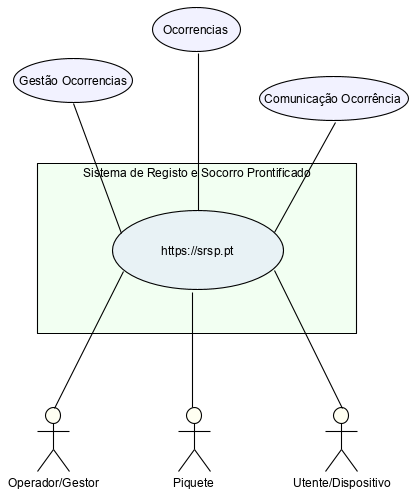
\includegraphics[width=0.55\textwidth]{figuras/cenario_global_sistema.png}
	\caption{Diagrama de casos de uso}
	\label{fig:cenario_global}
\end{figure}

\section{As 11 questões da análise de tarefas}

\subsection{Quem vai utilizar o sistema?}
\paragraph{Quem são:}Os utilizadores serão pessoas com mobilidade reduzida e em muitos casos vivem sozinhos.

\paragraph{Tipo de utilizadores:} Os utilizadores serão, na maioria dos casos, cidadãos seniores com pouco domínio das tecnologias, que vivem sozinho (tendo por isso pouca acesso ajuda na configuração e utilização do sistema) e com problemas de saúde de diversas naturezas, dos quais os mais significativos serão aqueles que causam imobilização ou a possibilidade de perda de sentidos.

\paragraph{Hábitos de trabalho:} Os utilizadores serão elementos que já não exercem trabalhos activos, estando em alguns casos confinados à sua habitação.

\paragraph{Aptidões:} A maior parte não possui qualquer tipo de hábito de trabalho com sistemas electrónicos, sendo mesmo uma franja da população conhecida por ter dificuldades nas utilizações mais simples destes tipos de sistemas.

\paragraph{Deficiências Físicas-motoras:} Os utilizadores terão diversos graus de incapacidade físico-motoras, no entanto partimos do princípio que a mais recorrente serão as dificuldades de locomoção, problemas de visão e de audição.


\subsection{Que tarefas executam actualmente?}
Os utilizadores já efectuam e recebem chamadas através de equipamentos montados nas suas residências, conhecem a utilização básica de um botão e compreendem a função do sistema de tele-assistência.

\subsection{Que tarefas são desejáveis?}
Activar o botão em casos de emergência, transportar o sistema de tele-assistência e ter a capacidade de reportar falsas pedidos de assistência.

\subsection{Como se aprendem as tarefas?}
O sistema poderá ser apresentado por um familiar/amigo do utilizador que domine este tipo de tecnologia com maior à vontade. E também desejável que sejam realizados um ou mais testes de utilização, de modo a confirmar a usabilidade do sistema e como treino para o utilizador.

\subsection{Onde são desempenhadas as tarefas?}
As tarefas serão desempenhadas na residência do utilizador e/ou num raio de até 100m, nomeadamente jardins, pátios, quintais ou zonas adjacentes á habitação.

\subsection{Quais são as relações entre utilizadores e informações?}
O sistema será acessível apenas através do hardware disponibilizado, sendo os dados acessíveis apenas relacionados com o mesmo.

\subsection{Que outros instrumentos tem o utilizador?}
O utilizador tem acesso a sistemas de telecomunicações típicos que se encontram nas residências (computadores, telefones fixos, telemóveis, etc…). Poderão ainda existir sistemas de alarmes de naturezas diversas, que já existam montados na residência

\subsection{Como comunica os utilizadores entre si?}
Os utilizadores comunicam com os contactos de emergência através de chamada de voz, sendo a chamada realizada por o contacto de emergência após uma notificação electrónica.

\subsection{Qual a frequência de desempenho de tarefas?}
Sendo este um sistema de tele-assistência em casos de emergência, parte-se do princípio que não haverá uma frequência especifica de utilização.

\subsection{Quais as restrições de tempo impostas?}
O sistema deverá ser célere na sua resposta uma vez que a sua utilização implica uma situação de emergência. Assim em condições ideais é desejável que as notificações destinadas ao contacto de emergência sejam inferiores a 30 segundos e que a resposta (chamada por parte do contacto de emergência) seja inferior a 5 minutos.

\subsection{Que acontece se algo corre mal?}
O sistema irá ser instalado numa unidade autónoma com capacidade de retenção de energia para operação continua durante pelo menos 1 semana (bateria interna), poderão ser adicionados outros sensores ao sistema (além do botão), tais como: sistema de alarme, detecção de incêndio/fumo, etc.

\section{Cenários do problema}

Todos os cenários terão como actor o Sr. Marques, um idoso que vive sozinho na sua casa. O Sr. Marques sofre de problemas musculares e demonstra inícios de uma doença degenerativa, que lhe afectam a mobilidade. Tendo trabalhado a vida inteira como coveiro num cemitério de minorias étnicas e como produtor de tofu vegano orgânico, possui pouco contacto com sistemas de tele-assistência. Devido ao avançado da sua idade, ao falecimento do seu companheiro de vida e o facto de os seus filhos adoptivos não estarem tão presentes quanto necessário, decidiu passar a utilizar um sistema de tele-assistência que possa comunicar eficazmente situações de emergência.

\subsection{Cenário de problema para a tarefa 1 – Reportar uma situação de emergência, através do botão de pânico}

O Sr. Marques devido à sua doença degenerativa possui perdas de memória e momentos de confusão e desorientação. Preocupado com o facto, de num dos seus episódios de confusão, puder ter ingerido uma linguiça de carne de porco em vez do seu tofu vegano orgânico, ficou preocupado que pudesse sofrer uma reacção alérgica. Não sabendo o que fazer e sentindo-se desesperado em não conseguir resolver o caso sozinho, decidiu activar o sistema de tele-assistência. Apesar de estar confuso e stressado com a situação, ao olhar para o mesmo verificou que havia apenas um botão vermelho de grandes dimensões. Sem ter grandes dúvidas, pois associou a cor do botão a uma situação de perigo, carregou no mesmo.
O sistema activou-se e registou uma situação de emergência assinalada pelo utilizador, despoletando uma notificação electrónica para os contactos de emergência do Sr. Marques.
Os contactos (que são os seus filhos), rapidamente, telefonaram ao Sr. Marques. Este como não estava incapacitado dirigiu-se ao telefone e atendou. Depois de uma pequena conversa os filhos perceberam a situação e acalmaram o pai, assegurando ao mesmo que ainda que ele tivesse ingerido uma linguiça não havia problema, pois o Sr. Marques não é alérgico à carne de porco.


\subsection{Cenário de problema para a tarefa 2 – Detectar uma potencial queda do utilizador}

Devido a possuir dificuldades de locomoção, o Sr. Marques escorregou no chão molhado da sua casa de banho. O Sr. Marques não se conseguia levantar sozinho pois as suas doenças degenerativas afectam-lhe a sua coordenação e capacidades motoras.
Devido ao facto de viver sozinho, não havia ninguém que tomasse conta do sucedido até a próxima visita de um dos seus familiares. Felizmente uma função no código do sistema de tele-assistência detectou, através do seu conjunto de sensores, uma possível queda do utilizador.
O sistema registou uma situação de emergência, despoletando automaticamente uma notificação electrónica para os contactos de emergência do Sr. Marques.
Esses contactos são os seus filhos, que ao receberem a notificação tentaram entrar em contacto com o Pai. O telefone do Sr. Marques tocou insistentemente, mas o estando caído na casa de banho não havia capacidade para o atender. Assim os filhos aperceberam-se que algo se passava e deslocaram-se imediatamente à residência do seu Pai, onde o encontraram caído na casa de banho. 


\subsection{Cenário de problema para a tarefa 3 – Monitorizar e detectar períodos de imobilização prolongados}

Com o passar do tempo os problemas degenerativos do Sr. Marques foram-se agravando, começando a afectar seriamente o controlo muscular e motor do Sr. Marques. Não era, pois, invulgar que de súbito o Sr. Marques perdesse controlo do seu corpo, ficando num estado de imobilidade involuntária.
Num desses ataques o Sr. Marques estava sentado na mesa da sua cozinha, onde tinha acabado a sua refeição de Tofu vegano orgânico. Incapaz de se movimentar e não havendo ninguém a quem pudesse requisitar ajuda o Sr. Marques ficou nesta situação durante 30 minutos. O sistema de tele-assistência, que estava com o Sr. Marques, através de uma função no seu código verificou que os seus sensores não detectavam alterações na sua posição ou aceleração à um período de 30 minutos. Emitiu por isso um aviso sonoro (através de um buzzer) para sinalizar que tinha verificado uma possível situação de perigo devido a imobilização prolongada. Este aviso servia, para o Sr. Marques mover o aparelho no caso de não se encontrar em perigo. Não possuindo essa capacidade e tendo passado mais 3 minutos sem haver movimentos significativos, o sistema despoletou uma notificação electrónica para os contactos de emergência do Sr. Marques. Os filhos receberam uma notificação electrónica e um link que abria um serviço de visualização de mapas, onde estava descrita a posição do sistema de teleassistência.
Os filhos apercebendo-se que o pai estava imobilizado deslocaram-se a casa do mesmo e tentaram ajudá-lo a recuperar os movimentos.


\subsection{Cenário de problema para a tarefa 4 – Reportar uma falsa detecção de situação de emergência}

O sr. Marques sempre foi um ávido espectador do concurso televisivo “Quem quer ser milionário”, chegando mesmo a exaltar-se com as respostas dadas pelos concorrentes. Numa das sessões do concurso a seguinte pergunta foi feita:

\begin{quote}
	“O Tofu vegano orgânico é produzido com base em … “
	
	”A. Milho transgénico;	B. Órgãos de carneiro picado; C. Soja orgânica; D. Tremoços”
\end{quote}

Tendo a certeza da resposta, o Sr. Marques no ímpeto do seu entusiasmo, clicou sobre o grande botão vermelho do sistema de tele-assistência (o qual imaginou como a campainha do jogador) e gritou a plenos pulmões:
\begin{quote}
	“RESPOSTA C, é feito com soja orgânica”
\end{quote}

Apercebendo-se imediatamente de que tinha activado o sistema de tele-assistência, o Sr. Marques iniciou os procedimentos para reportar remotamente uma falsa activação. Para tal pressionou o botão vermelho durante 15 segundos, o sistema emitiu dois sinais sonoros consecutivos, sinalizando que havia enviado de seguida uma notificação no qual informava os contactos de que tinha havido uma activação acidental do sistema e que o utilizador havia sinalizado a mesmo como falso positivo. 

\section{Caracterização dos actores}

O sistema vai funcionar com base em três tipos de actores.

\begin{itemize}
	\item\textbf{Gestor do sistema - }Tem como função gerir o sistema, garantindo a criação dos piquetes e fazendo a gestão das ocorrências.
	
	\item\textbf{Utente do sistema - }Tem como função criar as ocorrências.
	
	\item\textbf{Piquete - }Tem como função receber os avisos das ocorrências e prestar o auxílio necessário. Pode-se dizer que no âmbito do sistema a desenvolver, este será o actor mais passivo, uma vez que a sua única função é responder ao sistema.
\end{itemize}

\section{Caracterização das tarefas}

Tendo em vista a criação do sistema desde raiz, torna-se necessário ter atenção a dois conjuntos de tarefas, as que envolvem a gestão do sistema e as que envolvem a utilização do hardware. A gestão do sistema é necessariamente anterior à utilização do sistema.
\begin{itemize}
	\item\textbf{Criação de um piquete -} O gestor do sistema deve criar um, ou mais, entidades que recebem os avisos de ocorrências (piquete) por parte do sistema. A esta entidade deve estar associado uma séria de informações que garantam a capacidade de contacto. 
	
	\item\textbf{Reportar uma ocorrência manualmente -} Uma ocorrência pode ser reportada pelo utilizador, de modo consciente, através do pulsar de um botão de pânico que está associado ao sistema.
	
	\item\textbf{Reportar uma ocorrência automaticamente -} Uma ocorrência pode também ser reportada sem acção consciente do utilizador, através dos sensores associados ao sistema. 
	
	\item\textbf{Receber o aviso de uma ocorrência -} O piquete que se encontre na zona da ocorrência recebe automaticamente um aviso electrónico.
	
\end{itemize}

\section{Diagramas de casos de uso}

Para descrever os principais casos de uso do sistema, utilizou-se o diagrama de casos de uso presente na \ref{fig:diagrama_casos_uso}. Podemos observar nesta figura a interacção entre elementos do sistema num contexto de
elevada abstracção. Os principais casos descritos no âmbito dese trabalho são:
\begin{itemize}
	\item Adicionar piquete, por parte do gestor do sistema;
	\item Utilização do botão de SOS, por parte do utente do sistema;
	\item Detecção de queda do utente do sistema;
	\item Envio de um alerta de ocorrência para o piquete;
\end{itemize}

\begin{figure}[!htb]
		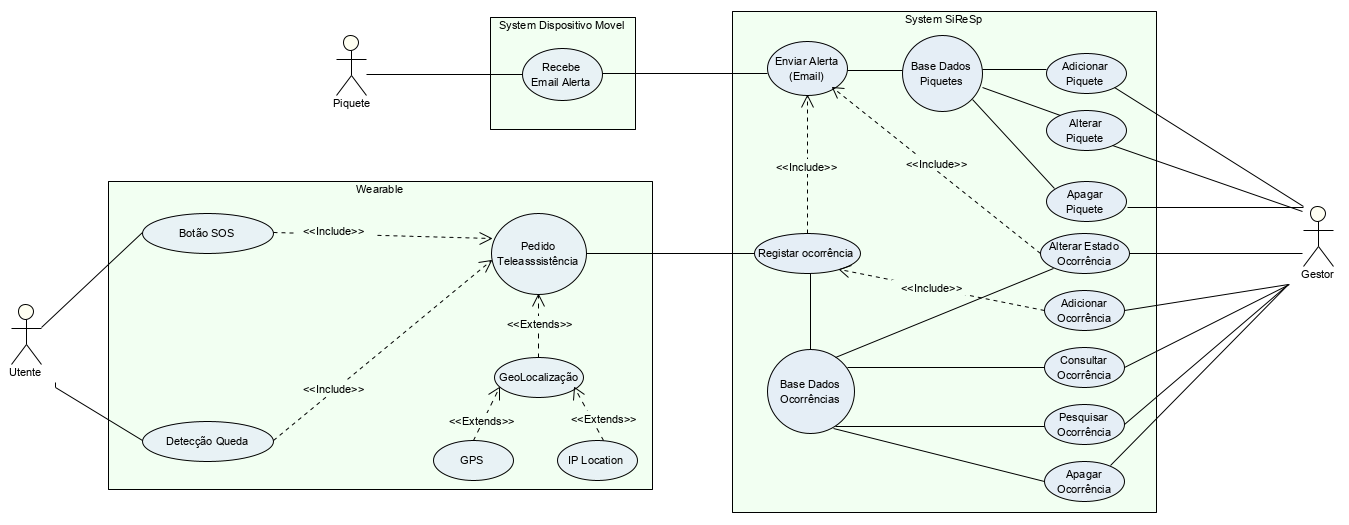
\includegraphics[width=\textwidth]{figuras/diagrama_casos_uso.png}
		\caption{Diagrama de casos de uso}
		\label{fig:diagrama_casos_uso}
\end{figure}

\section{Especificação dos casos de uso}

O cenário de utilização normal do sistema permite elaborar e ilustrar um caso de uso numa tabela, na qual são descritos os atributos do caso de uso, sequência e funcionalidades. Na tabela \ref{tab:exemplo_caso_uso}, apresentamos o exemplo do nosso primeiro caso de uso - "adicionar um piquete".

% usamos o pacote "\usepackage[section]{placeins}" com a opção [h] na tabela para aforçar a ficar na secção a que pertence
\begin{table}[h]
	\caption{Exemplo de caso de uso}
	\label{tab:exemplo_caso_uso}
	\centering
\begin{tabular}{
		|>{\centering\arraybackslash}m{3.5cm}
		|>{\centering\arraybackslash}m{0.5cm}
		|>{\arraybackslash}m{5cm}
		|>{\arraybackslash}m{5cm}
		|
	}
%\begin{tabular}{|>{\centering\arraybackslash}m{3.5cm} |m{0.5cm}	|m{5cm}	| m{5cm} | }
	\hline
	\textbf{Caso de uso}                           & \multicolumn{3}{l|}{Adicionar piquete.}
	\\ \hline
	\textbf{Nota}                                  & \multicolumn{3}{l|}{Neste cenário o utilizador representa o gestor do sistema.}
	\\ \hline
	\textbf{Breve descrição}                       & \multicolumn{3}{l|}{O gestor de sistema vai criar um novo piquete.}
	\\ \hline
	\textbf{Pré-condições}                         & \multicolumn{3}{p{11cm}|}{O gestor deve estar autenticado no sistema, situar-se na homepage e possuir as informações correctas.}
	\\ \hline
	\textbf{Pós-condições}                         & \multicolumn{3}{l|}{As informações do piquete passam a estar presentes no sistema.}
	\\ \hline
	\multirow{7}{*}{\rotatebox[origin=c]{90}{Sequência de eventos}} & \multicolumn{1}{c|}{}  & \multicolumn{1}{c|}{Input do actor} & \multicolumn{1}{c|}{Resposta do sistema}
										  \\ \cline{2-4} 
										  & \multicolumn{1}{c|}{1} & No menu de navegação, que se encontra no topo da página, clicar sobre a opção Piquetes & 
										  \\ \cline{2-4} 
										  & \multicolumn{1}{c|}{2} & &É apresentado a página de piquetes. Nesta página estão os botões “adicionar piquete” e “procurar”, bem como uma lista do piquetes já criados.
										  \\ \cline{2-4} 
										  & \multicolumn{1}{c|}{3} & Clicar sobre o botão “adicionar piquete” & 
										  \\ \cline{2-4} 
										  & \multicolumn{1}{c|}{4} &  & É apresentada uma página que contêm os campos “Zona”, “Nome”, “Email”, “Numero” e “Notas”. Existem também os botões “submit” e ”Cancel”
										  \\ \cline{2-4}
										  & \multicolumn{1}{c|}{5} & Preencher os campos com a as informações correctas e clicar no botão submit. & 
										  \\ \cline{2-4}										  
										  & \multicolumn{1}{c|}{6} &  & É apresentado, novamente, a página de piquetes. O piquete criado é apresentado no topo da página.
										  \\ \hline
\end{tabular}
\end{table}



\section{Requisitos}
\subsection{Requisitos funcionais}
\textbf{Botão de pânico/emergência:}o sistema deve ter um botão de emergência que efectua uma chamada de emergência para o número de assistência.
\\
\textbf{Receptor GPS:}o sistema deve ser capaz de saber a posição actual e enviá-la quando necessário (queda, botão, imobilização, …).
\\
\textbf{Sensor Acelerómetro:}o sistema tem de ter um sensor de queda.
\\
\textbf{Capacidade de análise:}o sistema deve saber quando o utilizador está imóvel demasiado tempo, por exemplo, após uma queda e imobilizado durante pelo menos 3 minutos.
\\
\textbf{Auto-diagnostico:}o sistema tem de avisar o utilizador quando a bateria está fraca abaixo de 25%.
\\
\textbf{Registo eventos Base Dados:}O sistema deve enviar para uma base de dados remota os pedidos de assistência (positivos e falsos positivos), posição, estado de bateria, etc…
\\
\textbf{Interface:} A interface tem de ser simples e para tal apenas deve ter duas luzes indicadoras de estado, verde e vermelho.

\subsection{Requisitos não funcionais}
\textbf{Desempenho:}o sistema deve ter um desempenho adequado, e permitir um envio de alerta em menos de 30 segundos.
\\
\textbf{Regras de utilização:}o sistema deve ser de utilização simples e intuitiva, adequada ao tipo de utilizador a que se destina.
\\
\textbf{Disponibilidade:}O sistema deve manter uma disponibilidade total de 99,9\%. 
\\
\textbf{Preço:}O sistema deve ter um custo inicial de desenvolvimento inferior a \euro25000, um custo de produção de hardware (dispositivo wereable) inferior a \euro100 e um custo de manutenção anual inferior a \euro50000 para o serviço de teleassistência.
\\
\textbf{Legislação:}deve ser implementado o Regulamento Geral sobre a Protecção de Dados

\subsection{Requisitos de desenvolvimento}
\textbf{Web Responsive:}desenvolvimento web responsive com suporte para vários dispositivos.
\\
\textbf{Linguagens de programação:}devem ser utilizadas as linguagens (não exclusivamente): C, PHP, HTML, SQL.
\\
\textbf{Servidores:}os servidores de registo de eventos devem utilizar os sistemas operativos Windows ou Linux.
\\
\textbf{Implementação/manutenção:}deve ser possível implementar novas funcionalidades através de updates Over the Air (OTA).